% IEEE standard conference template; to be used with:
%   spconf.sty  - LaTeX style file, and
%   IEEEbib.bst - IEEE bibliography style file.
% --------------------------------------------------------------------------

\documentclass[letterpaper]{article}
\usepackage{spconf,amsmath,amssymb,graphicx}
\usepackage[outdir=./]{epstopdf}
\usepackage{grffile}
\usepackage{url}
\usepackage{pgfplots}
\usepackage{pgf}
\usepackage{tikz}
\usepackage{caption}
\usepackage{subcaption}
\usepackage{listings}

\definecolor{verylightgray}{rgb}{0.92,0.92,0.92}
\definecolor{lightgray}{rgb}{0.75,0.75,0.75}
\definecolor{o_blue}{rgb}{0.0,0.5,1.0}

% Example definitions.
% --------------------
% nice symbols for real and complex numbers
\newcommand{\R}[0]{\mathbb{R}}
\newcommand{\C}[0]{\mathbb{C}}

% bold paragraph titles
\newcommand{\mypar}[1]{{\bf #1.}}

% Title.
% ------
\title{Lock-Free Concurrent Priority Queue}
%
% Single address.
% ---------------
\name{Renato Marroqu\'in, Aristeidis Mastoras, David Sidler} 
\address{Department of Computer Science\\ ETH Z\"urich\\Z\"urich, Switzerland}

% For example:
% ------------
%\address{School\\
%		 Department\\
%		 Address}
%
% Two addresses (uncomment and modify for two-address case).
% ----------------------------------------------------------
%\twoauthors
%  {A. Author-one, B. Author-two\sthanks{Thanks to XYZ agency for funding.}}
%		 {School A-B\\
%		 Department A-B\\
%		 Address A-B}
%  {C. Author-three, D. Author-four\sthanks{The fourth author performed the work
%		 while at ...}}
%		 {School C-D\\
%		 Department C-D\\
%		 Address C-D}
%

\begin{document}
%\ninept
%
\maketitle
%

%The hard page limit is 6 pages in this style. Do not reduce font size or use other tricks to squeeze. This pdf is formatted in the American letter format, so may look a bit strange when printed out.

\begin{abstract}

A priority queue appears in various multithreading applications.
%TODO . Being a challenge in practice has nothing to with mutual exclusion strategies
However, an efficient implementation for a concurrent priority queue is challenging in practice, since already proposed mutual exclusion strategies cause blocking and have bad scalability.\\
We present a lock-free implementation of a concurrent priority queue which only makes use of atomic operations which are present in most modern x86 CPUs.
The underlying data structure is a skip list enabling lookups in $\Theta(\log(n))$ and \textit{pop} operations in $\Theta(1)$ time complexity.\\
Experiments were conducted on a Xeon CPU and a Xeon Phi, we evaluated the difference between those platforms and also in comparison to different baseline implementations, e.g. Intel TBB priority queue [REF].
The experimental results show that our lock-free implementation is competitive against other implementations and even surpasses the baseline implementations in certain operations.

\end{abstract}


\section{Introduction}\label{sec:intro}

A priority queue is an abstract data structure, where all the elements in it are associated with a priority key.
Therefore, there is an order between all elements which is determined by this key. % THIS IS TOO DETAIL ... a default or custom comparator function.
Priority queues have two main operations: \textit{push} to insert elements and \textit{pop} to dequeue the element with the highest priority.
The priority queue guarantees that the element dequeued by a \textit{pop} operation has the highest priority.
Elements of equal priority are usually allowed and do not pose a problem.
A number of well known applications (e.g. job scheduling, constraint systems, Dijkstra's algorithm, and encoding algorithms) use a priority queue.
Hence, many different single-threading implementations have been proposed.

In recent years, CPU architecture have moved from single core to multi core systems.
Therefore, the research community has focused on parallelization of single-threading applications and the implementation of efficient concurrent data structures.
In a multi-threading application, multiple threads might access a priority queue simultaneously.
To guarantee consistency, the data structure has to be thread-safe.
One way to achieve thread-safety is mutual exclusion through structures e.g. locks, semaphores and other primitives.
All these methods cause blocking and only a single thread, the one in the critical region, might make progress.
Consequently, this approach limits scalability.\\
Another way to achieve thread-safety are lock-free data-structures which guarantee that no thread is blocked and at least one thread makes progress at any time.
Apart from a high implementation complexity and challenging correctness verification, this approach is in theory superior to naive mutual exclusion.
Atomic synchronization primitives which are necessary for a lock-free implementation are available on most modern x86 CPUs.\\
In this paper, we present a lock-free concurrent priority queue which exploits the characteristics of the underlying data structure.
A skip list \cite{Pugh:1990:SLP:78973.78977} is appropriate for a lock-free implementation thanks to its simplicty.
It provides probabilistic balancing using multiple levels, maintaining an ordered list of keys which provides fast \textit{pop} operations.\\
A heap-based concurrent priority queue which is designed for CUDA data parallel SIMT architecture is presented in \cite{DBLP:conf/hipc/HeAP12}.
The authors use wide heap nodes in order to support thousands of push and pop operations at the same time.
Sundell et al.~\cite{Sundell:2005:FLC:1073765.1073770} present a lock-free concurrent priority queue which uses a skip list, as the underlying data structure. Their implementation was evaluated on Pentium II architecture using up to 30 threads. In this paper a similar lock-free implementation is evaluated on a state-of-art CPU and a MIC architecture.\\
This paper is structured as follows.
Section~\ref{sec:background} gives a description of priority queues and skip lists.
Our implementation is presented in detail in section~\ref{sec:approach}. Section~\ref{sec:exp} describes experimental results collected from a Xeon CPU and Xeon Phi, by comparing the lock-free implementation with the Intel Threading Building Blocks (TBB) concurrent priority queue, and two different implementations using mutual exclusion. Finally, section~\ref{sec:con} concludes this work.


\section{Background: Whatever the Background is}\label{sec:background}

A priority queue is an abstract data structure which can be implemented using various data structures.
An efficient implementation can be achieved with a heap which is based on an array.
t requires $\mathcal{O}(\log{}n)$ time complexity for both operations, \textit{insert} and \textit{deleteMin}, and $\mathcal{O}(n)$ space complexity.
Nevertheless, other implementations may provide faster operations thanks to time complexity, space complexity and data locality.

Our lock-free implementation is based on a skip list which provides probabilistic balancing.
The bottom level is an ordinary ordered linked list, and each of the other levels acts as a subset of the elements of the lower levels which assist in faster operations.
Each element of a level \textit{i} appears on the level \textit{i+1} with probability 0.5.
Therefore, the first level contains all the elements, the second one contains 50\% of them, the third one 25\% and so on.

A skip list requires more memory than other data structures (e.g a heap which is implemented using an array), since every node has multiple pointers to the next node.
However, it supports the \textit{deleteMin} operation in $\Theta(1)$, since the elements are ordered and the element with the maximum priority is located always in the beginning.
The time complexity for the \textit{insert} is $\mathcal{O}(\log{}n)$.


%Give a short, self-contained summary of necessary background information. For example, assume you present an implementation of FFT algorithms. You could organize into DFT definition, FFTs considered, and cost analysis. The goal of the background section is to make the paper self-contained for an audience as large as possible. As in every section you start with a very brief overview of the section. Here it could be as follows: In this section we formally define the discrete Fourier transform, introduce the algorithms we use and perform a cost analysis.

%\mypar{Discrete Fourier Transform}
%Precisely define the transform so I understand it even if I have never seen it before.

%\mypar{Fast Fourier Transforms}
%Explain the algorithm you use.

%\mypar{Cost Analysis}
%First define you cost measure (what you count) and then compute the cost. Ideally precisely, at least asymptotically. In the latter case you will need to instrument your code to count the operations so you can create a performance plot.

%Also state what is known about the complexity (asymptotic usually) about your problem (including citations).
%Don't talk about "the complexity of the algorithm.'' It's incorrect, remember (Lecture 2)?

%\begin{itemize}
%	\item Priority queue theory/use cases.
%	\item Existing research on priority queues.
%	\item Do complexity analysis for underlying data structures.
%	\item Lock-free data structures for ppq
%\end{itemize}


\section{Proposed Approach}\label{sec:approach}


\begin{itemize}
	\item Lock-based implementation
	\item Lock-free implementation
	\item Correctness tests with applications
	\item Explain advantages vs disadvantages of approach
\end{itemize}

We decided to base the implementation of our concurrent priority queue on a lockfree Skiplist. A lockfree Skiplist is a good choice for a concurrent datastructure since the atomic operations are very local to 2-3 nodes and thereby the probabilty of conflicts between threads is minimized. Since our final goal was a port on to the Xeon Phi which comes with 60 cores this would be a good fit.\\
The Skiplist was implemented using C++ atomics and its {\em comapre\_and\_exchange} operation.\\
In Figure XX we have an illustration of Skiplist which essentially is a linked list with a hierarchial tree-like index structure. The index creation is probabilistic but should asymptotically lead to a structure which enables traversing to any node in $O(\log n)$.\\
MAYBE EXPLAIN some operations\\
Like most lockfree data structures we had to deal with the problem {\em predecessor-deletion} [FIND BETTER WORD, see paper]. The problem is explained in figure XX.
A common resolution is to add a delete flag to each node for lazy deletion. But this means it is necessary to do CAS operation on the {\em next} pointer and the delete flag simulatenously. Multiple options are possible: {\em Atomic Markable Reference}, Double CAS, double-width CAS, Transactional-Memory. For our implementation we used the first option and implemented a {\em Atomic Markable Reference} by using the least significant bit as a deletion flag. Thereby we are able to use the general {\em compare\_and\_exchange} operation in C++11. Since our next pointers are always alligned to 64bytes [what is the architecture doing??]. In general no issues should arise when using the least significant bit as a deletion flag.\\
Apart from the common Skiplist methods: empty(), size(), find(), remove(), insert(). We added a pop() method necessary for a priority queue and pop(k) and insert(k) for batch processing.\\


%MAYBE give complete API somewhere
\begin{lstlisting}[language=C++,basicstyle=\tt\footnotesize,captionpos=b,caption=PPQ interface,morekeywords={*, size_t}]
template <class T, class Comp> class PPQ
{
	bool empty() const;
	size_t size() const;
	bool push(const T& data);
	size_t push(T data[], int k);
	bool remove(const T& data);
	bool pop_front(T& data);
	size_t pop_front(T data[], int k);
	bool contains(T data);
	void print();
};
\end{lstlisting}

\subsection{Correcteness verification}
\label{subsec:corr_ver}
We used two different applications for verifying the correctness of our algorithm, a loseless data compression algorithm and an algorithm to find the shortest path in a graph. 
%\mypar{Huffman coding algorithm}
We implemented the Huffman coding algorithm as an initial correcteness test for our data structure implementation. This algorithm consists in two main steps. The first step is to initialize a data structure which keeps all the items sorted by their frequency. Then in a second step, it iterates until the data structure has a single element. Every iteration consists of picking the two nodes with the lowest frequency/probability, creating a parent node out of them with the sum of the children's frequencies/probabilities, inserting this new node into the data structure and assigning code zero, or one to the children, and delete them from the data structure. We compared the output of a Huffman coding algorithm using a min-heap with an implementation using our priority queue. We only compared correctness between this two implementations as this loseless compression algorithm is based on iterating linearly through the elements of the underlying data structure and no concurrent access is done.
%\mypar{Shortest path algorithm}
A shortest path algorithm performs searches over a graph to determine the a path with the least number of hops between two nodes. Thus, we tested the correctness of our application against the shortest path algorithm implementation provided by Intel TBB. This implementation uses Intel TBB concurrent priority queue by default, and we adapted to also use our priority queue. We verified the correctness of both outputs. We didn't measure any performance over these algorithms as this might have implied some specific tuning for each of them. This falls out of the scope of this project. In section~\ref{sec:exp}, we do performance evaluation against Intel TBB concurrent priority queue with specific workloads.

\subsection{Memory allocation micro-benchmark}
We performed a microbenchmark to evaluate the memory allocation process in the XeonPhi. We did three different types of mememory allocation: First, we used the primites offered by the programming language, then we used compiler hints offered by the Intel Thread Building Blocks to use its scalable allocator implementation, and finally we allocated the memory needed sequentially using compiler hints too. These options are described below.

\mypar{C++ memory allocation primitives}
These are optimized for sequential case. They were designed with two main objectives: use efficiently memory space and minimize CPU overhead. However, these objectives do not target achieving good parallel performance. Modern hardware provides larger memory sizes, but also a bigger gap between CPU and memory speed. Thus, cache locality and avoidance of false sharing play a more important role.

\mypar{Intel TBB scalable allocator}
It uses \textit{thread-private heaps} to reduce the amount of code that needs synchronization and also false sharing. Each thread allocates its own copy of heap structures and accesses it via thread-specific data (TSD) using corresponding system APIs.
The allocator gets 1MB chunks from the operating system and divides them into 16K-byte aligned blocks. Then, it places these blocks initially in a global heap of free blocks. Memory requested is not returned to the operating system (but only in large allocation cases). Thus, it can make sure that memory is reused. Additional blocks are requested if a thread does not find free objects in the blocks of its own heap and there are no available blocks in the global heap~\cite{_thefoundations,Hudson:2006:MST:1133956.1133967}.
To use the scalable allocator offered by Intel TBB we had to link two libraries:
\begin{description}
	\item[-ltbb] To use the Intel TBB library.
	\item[-ltbbmalloc] To use the scalable allocator offered by the Intel TBB library.
\end{description}
 
\mypar{Sequential allocation with compiler hints}
Every node in our skip list contains an array of pointers to the next nodes depending on the level each node belongs to. This means that parts of this array might fall into different cache lines. Thus, our data structure can suffer more from cache misses and false sharing. We designed each skip list node to contain an empty array and allocating only the pointers that it will actually need (listing~\ref{lst:freenode}). In addition to that, the usage of Intel TBB allocator helps us ensuring that these nodes will be cache-aligned (listing~\ref{lst:fn_alloc}).

\begin{lstlisting}[language=C++,basicstyle=\tt\footnotesize,captionpos=b,caption=Lock free node structure,label=lst:freenode,morekeywords={*, size_t}]
template <typename T>  struct LockFreeNode
{	
	T data;
	int	level;
	AtomicRef<LockFreeNode>	next[0];
};
\end{lstlisting}

\begin{lstlisting}[language=C++,basicstyle=\tt\footnotesize,captionpos=b,caption=Memory allocation instruction for array of atomic references,label=lst:fn_alloc, morekeywords={*, size_t}]

scalable_malloc(
sizeof(LockFreeNode) 
+ 
((arrayLength + 1) * sizeof(AtomicRef<LockFreeNode>))
)
\end{lstlisting}

\mypar{Memory allocation microbenchmnark}
We designed our microbenchmark to allocate ten million skip list nodes while using 240 threads. We measured the time it takes to complete the allocation task on the XeonPhi. When using the regular memory allocation method, we experienced really high latency but when we used Intel TBB scalable allocator we obtained a 24, and 38 times improvemente for using TBB library, and a sequential allocation with Intel TBB allocator respectively. The results are displayed on figure~\ref{fig:mem_alloc}.


% explain data + graph 
\begin{figure}
	\centering
  	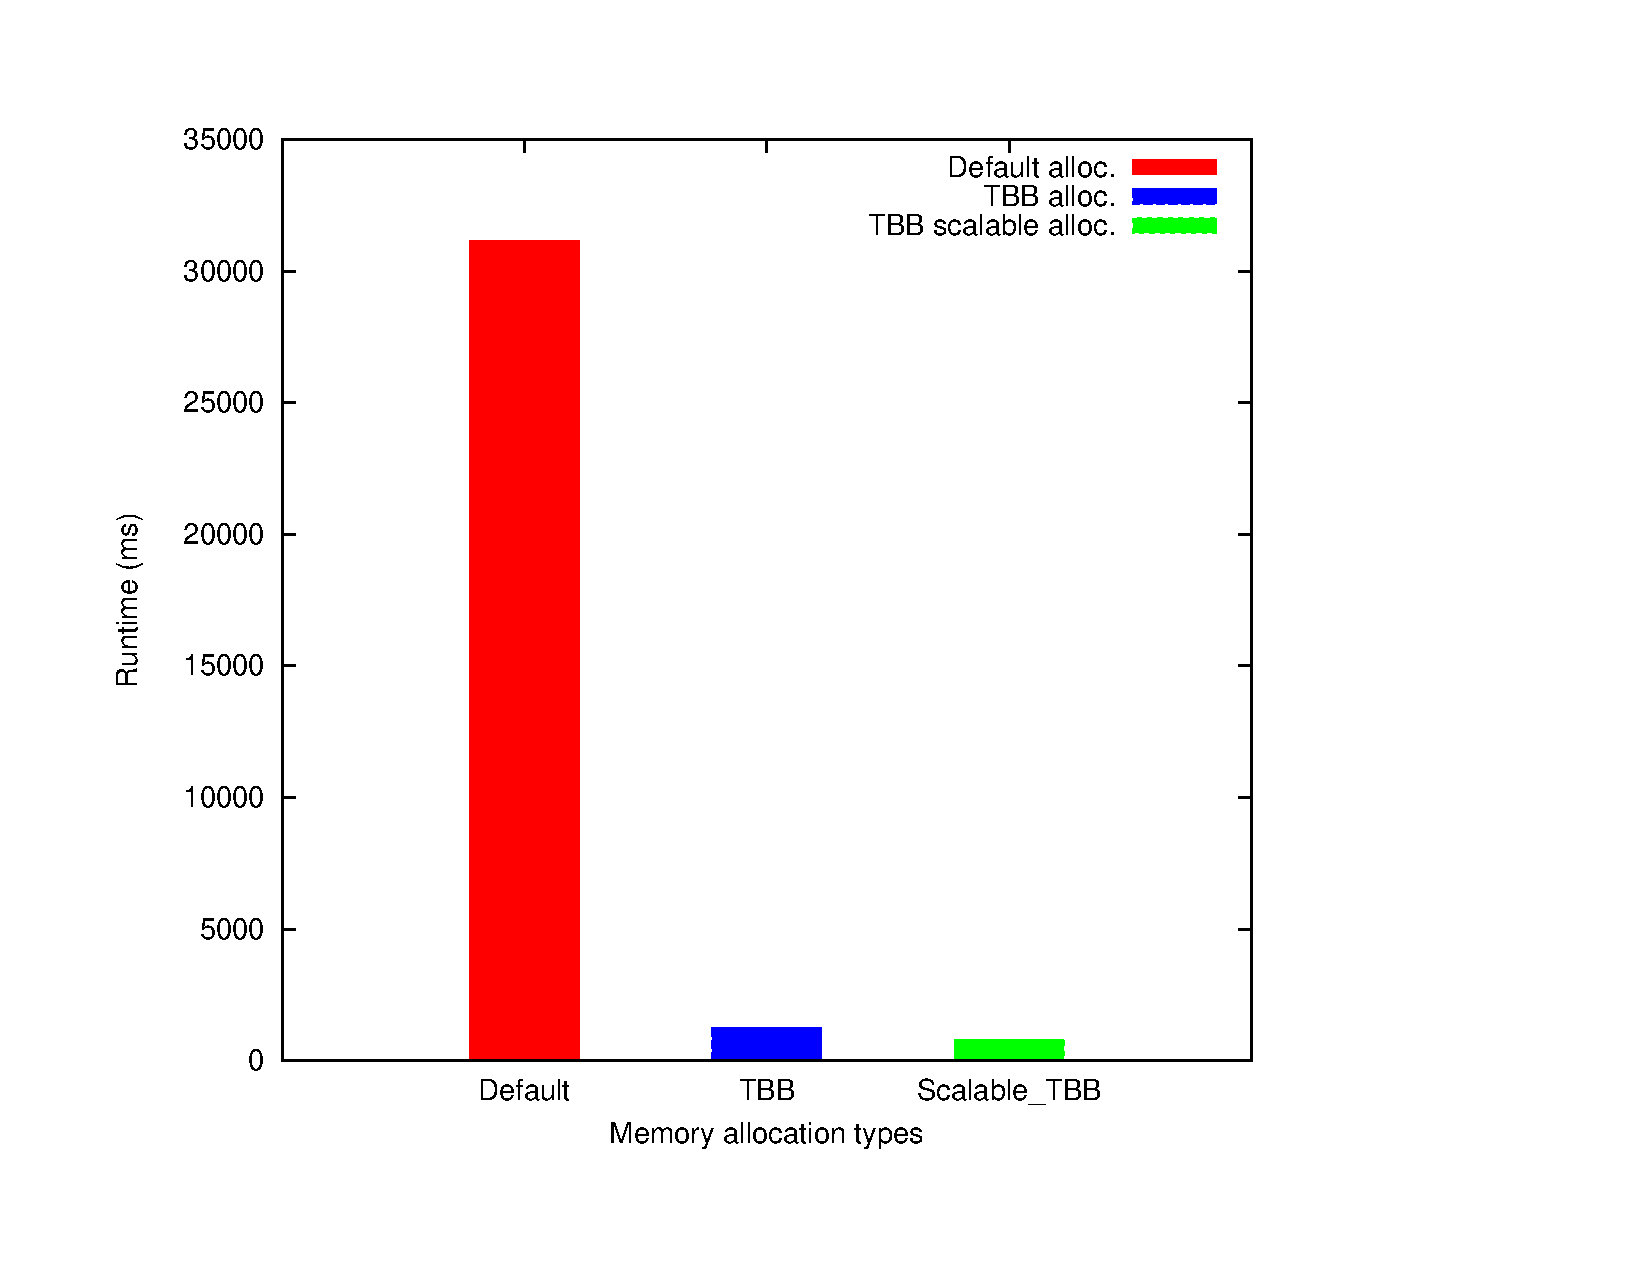
\includegraphics[scale=0.35]{../plots/mem_alloc/mem_alloc.pdf}
	\caption{Memory allocation runtime among a regular allocation, using compiler hints, and using sequential allocation with compiler hints}
	\label{fig:mem_alloc}
\end{figure}


\section{Experimental Results}
\label{sec:exp}
\subsection{Evaluation on Workloads}
The experiments were conducted on two different systems. First, a CPU-based system equipped with an Intel Xeon E3-1245 running 4 cores at 3.4\,Ghz and 24\,GB main memory. Second a MIC, the Intel Xeon Phi 7120P which has 60 cores with 4 hyper-threads, each clocked at 1.23\,Ghz. It also has 16\,GB main memory with a bandwidth of 352\,GB/s. To allow a comparison, the experiment parameters used were the same on both platforms. For each experiment five iterations were averaged and their standard deviation was computed.

Three types of workload were executed, \textit{mixed}, \textit{push} and \textit{pop}. For the mixed and pop, the concurrent priority queue was prepopulated with 1000$\times$threads in the former and 10\,Mio. elements in the latter. Prepopulation was not included in the measured runtime. The \textit{mixed} workload chooses for each operation with a probability of 50\% either a \textit{push} or \textit{pop} operation. The number of threads is increased from 1 to 240, in steps of 20, while the number of operations per threads stays constant.

\subsubsection{Evaluation on Xeon Haswell}
\begin{figure*}[t]
	\centering
	\begin{subfigure}[b]{0.3\textwidth}
		\centering
		%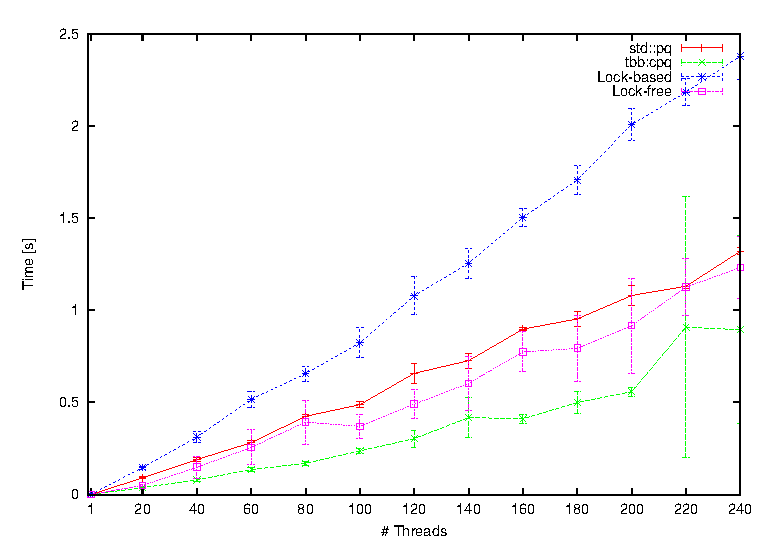
\includegraphics[width=\textwidth]{../plots/i7_mixed/runtime_mixed_i7}
		\begin{tikzpicture}
\begin{axis}[
width=2.5in,
xlabel={\#Threads},
ylabel={Time [s]},
xmin=-10,
xmax=250,
xtick={0,80,...,240},
ytick={0, 500, 1000, 1500, 2000},
yticklabels={0, 0.5, 1, 1.5, 2},
ymin=0,
ymax=2000,
scaled x ticks = false,
legend style={at={(0.05,0.95)},anchor=north west, font=\tiny}]

\addplot[mark=*,blue, mark size=1.5]
table[x=Threads,y=std,col sep=comma] {../plots/xeon_mixed/xeon_mixed.csv}; 
\addlegendentry{std::pq}

\addplot[color=red,mark=triangle*, mark size=2]
table[x=Threads,y=tbb,col sep=comma] {../plots/xeon_mixed/xeon_mixed.csv}; 
\addlegendentry{tbb::cpq}

\addplot[color=brown,mark=square*, mark size=1.5]
table[x=Threads,y=lb,col sep=comma] {../plots/xeon_mixed/xeon_mixed.csv}; 
\addlegendentry{Lock-based}

\addplot[color=darkgreen,mark=diamond*, mark size=2]
table[x=Threads,y=lf,col sep=comma] {../plots/xeon_mixed/xeon_mixed.csv}; 
\addlegendentry{lock-free}

\end{axis}
\end{tikzpicture}
		\caption{Mixed workload}
		\label{fig:xeon_mixed}
	\end{subfigure}
	\hfill
	\begin{subfigure}[b]{0.3\textwidth}
		\centering
		\begin{tikzpicture}
\begin{axis}[
width=2.5in,
xlabel={\#Threads},
ylabel={Time [s]},
xmin=-10,
xmax=250,
xtick={0,80,...,240},
ytick={0, 1000, 2000, 3000, 4000},
yticklabels={0, 1, 2, 3, 4},
ymin=0,
ymax=4500,
scaled x ticks = false,
y label style={at={(0.1,0.5)}},
legend style={at={(0.05,0.95)},anchor=north west, font=\tiny}]

\addplot[mark=*,blue, mark size=1.5]
table[x=Threads,y=std,col sep=comma] {../plots/xeon_push/xeon_push.csv}; 
\addlegendentry{std::pq}

\addplot[color=red,mark=triangle*, mark size=2]
table[x=Threads,y=tbb,col sep=comma] {../plots/xeon_push/xeon_push.csv}; 
\addlegendentry{tbb::cpq}

\addplot[color=brown,mark=square*, mark size=1.5]
table[x=Threads,y=lb,col sep=comma] {../plots/xeon_push/xeon_push.csv}; 
\addlegendentry{Lock-based}

\addplot[color=darkgreen,mark=diamond*, mark size=2]
table[x=Threads,y=lf,col sep=comma] {../plots/xeon_push/xeon_push.csv}; 
\addlegendentry{lock-free}

\end{axis}
\end{tikzpicture}
		\caption{Push workload}
		\label{fig:xeon_push}
	\end{subfigure}
	\hfill
	\begin{subfigure}[b]{0.3\textwidth}
		\centering
		%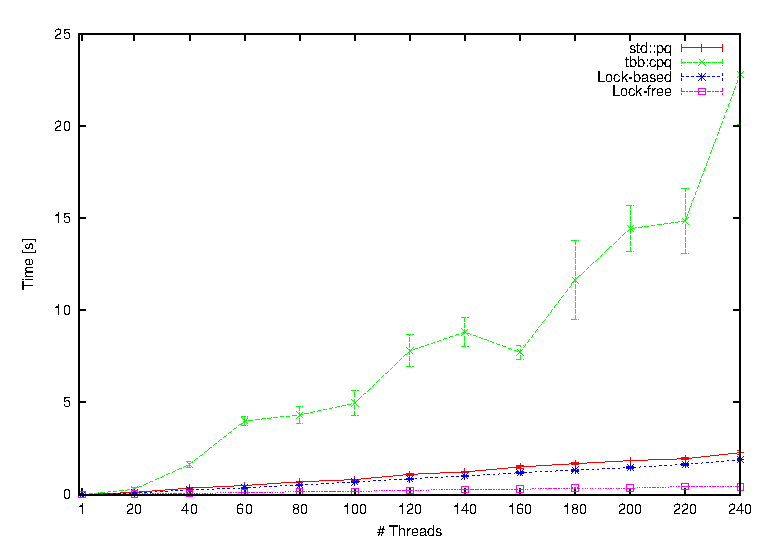
\includegraphics[width=\textwidth]{../plots/i7_pop/runtime_pop_i7}
		\begin{tikzpicture}
\begin{axis}[
width=2.5in,
xlabel={\#Threads},
ylabel={Time [s]},
xmin=-10,
xmax=250,
xtick={0,80,...,240},
ytick={0, 500, 1000, 1500},
yticklabels={0, 0.5, 1, 1.5},
ymin=0,
ymax=1500,
scaled x ticks = false,
legend style={at={(0.05,0.95)},anchor=north west, font=\tiny}]

\addplot[mark=*,blue, mark size=1.5]
table[x=Threads,y=std,col sep=comma] {../plots/xeon_pop/xeon_pop.csv}; 
\addlegendentry{std::pq}

\addplot[color=red,mark=triangle*, mark size=2]
table[x=Threads,y=tbb,col sep=comma] {../plots/xeon_pop/xeon_pop.csv}; 
\addlegendentry{tbb::cpq}

\addplot[color=brown,mark=square*, mark size=1.5]
table[x=Threads,y=lb,col sep=comma] {../plots/xeon_pop/xeon_pop.csv}; 
\addlegendentry{Lock-based}

\addplot[color=darkgreen,mark=diamond*, mark size=2]
table[x=Threads,y=lf,col sep=comma] {../plots/xeon_pop/xeon_pop.csv}; 
\addlegendentry{lock-free}

\end{axis}
\end{tikzpicture}
		\caption{Pop workload}
		\label{fig:xeon_pop}
	\end{subfigure}
	\caption{Runtime for different workloads executed on a Xeon E3-1245 while varying the number of threads}
	\label{fig:eval_i7}
\end{figure*}
Fig.~\ref{fig:eval_i7} shows the run-times for executing the three workloads on a Xeon E3-1245 system. All variants are performing and behaving similar in the \textit{mixed} and \textit{push} workload, except for the lock-based implementation which struggles more to scale with the number of threads. Our lock-free implementation is very close to the baseline implementations and shows similar behavior when increasing the number of threads. In the pop workload, all four data structures behave very similar.
The lock-free implementation with a \textit{pop} operation in $\Theta(1)$ and lazy-deletion shows the best runtime by a small margin.

\subsubsection{Evaluation on Xeon Phi}
\begin{figure*}[t]
	\centering
	\begin{subfigure}[b]{0.3\textwidth}
		\centering
		%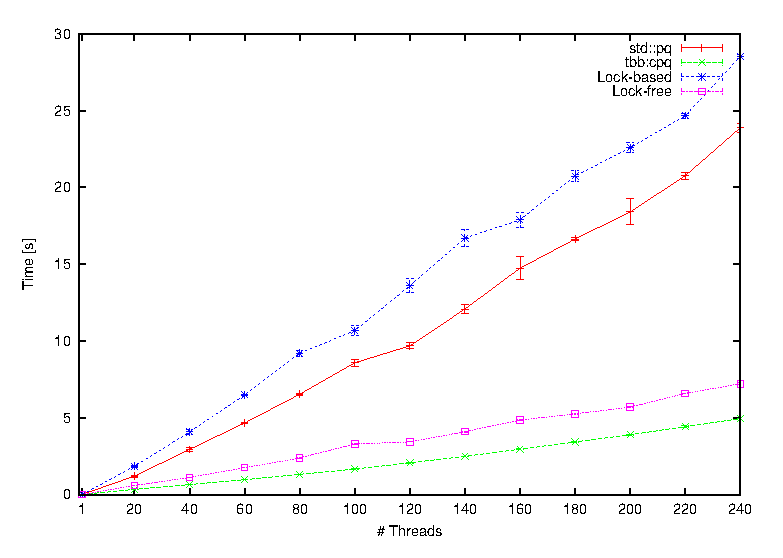
\includegraphics[width=\textwidth]{../plots/xp_mixed/runtime_mixed}
		\begin{tikzpicture}
\begin{axis}[
width=2.5in,
xlabel={\#Threads},
ylabel={Time [s]},
xmin=-10,
xmax=250,
xtick={0,80,...,240},
ytick={0,10000, 20000, 30000},
yticklabels={0, 10, 20, 30},
ymin=0,
ymax=30000,
scaled x ticks = false,
scaled y ticks = false,
y label style={at={(0.1,0.5)}},
legend style={at={(0.05,0.95)},anchor=north west, font=\tiny}]

\addplot[mark=*,blue, mark size=1.5]
table[x=Threads,y=std,col sep=comma] {../plots/xp_mixed/xp_mixed.csv}; 
\addlegendentry{std::pq}

\addplot[color=red,mark=triangle*, mark size=2]
table[x=Threads,y=tbb,col sep=comma] {../plots/xp_mixed/xp_mixed.csv}; 
\addlegendentry{tbb::cpq}

\addplot[color=brown,mark=square*, mark size=1.5]
table[x=Threads,y=lb,col sep=comma] {../plots/xp_mixed/xp_mixed.csv}; 
\addlegendentry{Lock-based}

\addplot[color=darkgreen,mark=diamond*, mark size=2]
table[x=Threads,y=lf,col sep=comma] {../plots/xp_mixed/xp_mixed.csv}; 
\addlegendentry{lock-free}

\end{axis}
\end{tikzpicture}
		\caption{Mixed workload}
		\label{fig:xp_mixed}
	\end{subfigure}
	\hfill
	\begin{subfigure}[b]{0.3\textwidth}
		\centering
		%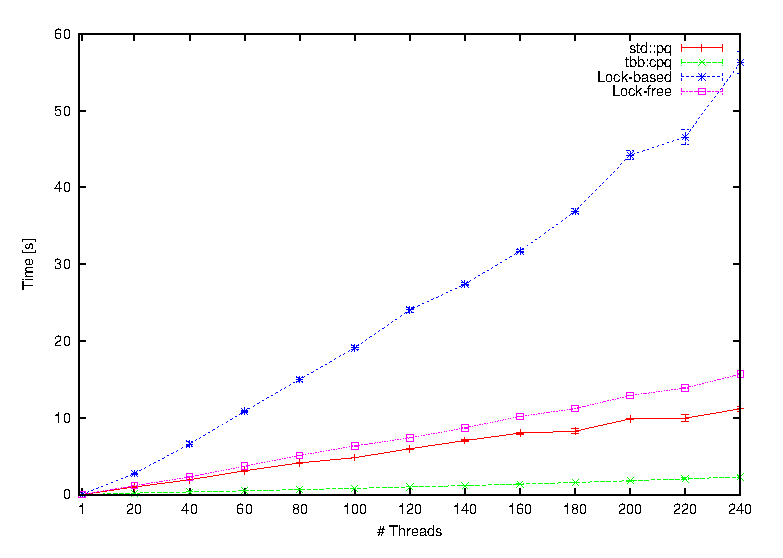
\includegraphics[width=\textwidth]{../plots/xp_push/runtime_push}
		\begin{tikzpicture}
\begin{axis}[
width=2.5in,
xlabel={\#Threads},
ylabel={Time [s]},
xmin=-10,
xmax=250,
xtick={0,80,...,240},
ytick={0, 15000, 30000, 45000, 60000},
yticklabels={0, 15, 30, 45, 60},
ymin=0,
ymax=60000,
scaled x ticks = false,
scaled y ticks = false,
y label style={at={(0.1,0.5)}},
legend style={at={(0.05,0.95)},anchor=north west, font=\tiny}]

\addplot[mark=*,blue, mark size=1.5]
table[x=Threads,y=std,col sep=comma] {../plots/xp_push/xp_push.csv}; 
\addlegendentry{std::pq}

\addplot[color=red,mark=triangle*, mark size=2]
table[x=Threads,y=tbb,col sep=comma] {../plots/xp_push/xp_push.csv}; 
\addlegendentry{tbb::cpq}

\addplot[color=brown,mark=square*, mark size=1.5]
table[x=Threads,y=lb,col sep=comma] {../plots/xp_push/xp_push.csv}; 
\addlegendentry{Lock-based}

\addplot[color=darkgreen,mark=diamond*, mark size=2]
table[x=Threads,y=lf,col sep=comma] {../plots/xp_push/xp_push.csv}; 
\addlegendentry{lock-free}

\end{axis}
\end{tikzpicture}
		\caption{Push workload}
		\label{fig:xp_push}
	\end{subfigure}
	\hfill
	\begin{subfigure}[b]{0.3\textwidth}
		\centering
		%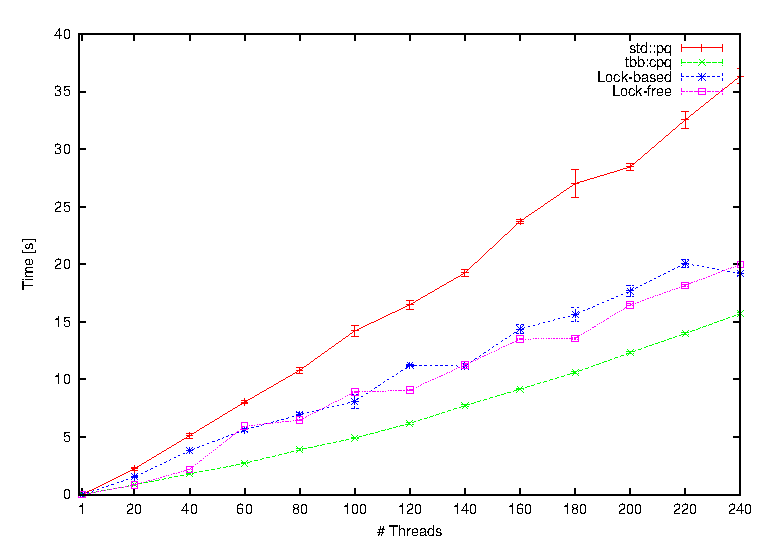
\includegraphics[width=\textwidth]{../plots/xp_pop/runtime_pop}
		\begin{tikzpicture}
\begin{axis}[
width=2.5in,
xlabel={\#Threads},
ylabel={Time [s]},
xmin=-10,
xmax=250,
xtick={0,80,...,240},
ytick={0, 10000, 20000, 30000, 40000},
yticklabels={0, 10, 20, 30, 40},
ymin=0,
ymax=40000,
scaled x ticks = false,
scaled y ticks = false,
y label style={at={(0.1,0.5)}},
legend style={at={(0.05,0.95)},anchor=north west, font=\tiny}]

\addplot[mark=*,blue, mark size=1.5]
table[x=Threads,y=std,col sep=comma] {../plots/xp_pop/xp_pop.csv}; 
\addlegendentry{std::pq}

\addplot[color=red,mark=triangle*, mark size=2]
table[x=Threads,y=tbb,col sep=comma] {../plots/xp_pop/xp_pop.csv}; 
\addlegendentry{tbb::cpq}

\addplot[color=brown,mark=square*, mark size=1.5]
table[x=Threads,y=lb,col sep=comma] {../plots/xp_pop/xp_pop.csv}; 
\addlegendentry{Lock-based}

\addplot[color=darkgreen,mark=diamond*, mark size=2]
table[x=Threads,y=lf,col sep=comma] {../plots/xp_pop/xp_pop.csv}; 
\addlegendentry{lock-free}

\end{axis}
\end{tikzpicture}
		\caption{Pop workload}
		\label{fig:xp_pop}
	\end{subfigure}
	\caption{Runtime for different workloads executed on a Xeon Phi while varying the number of threads}
	\label{fig:eval_xp}
\end{figure*}
The same workloads were also run on Xeon Phi. The measured run-times are plotted in Fig.~\ref{fig:eval_xp}.
In the mixed workload the TBB and the lock-free concurrent priority queue behave similarly well. The other two implementations show clearly a longer runtime.
%FIXME WHAT IS rsp?
Looking at the \textit{push} rsp. \textit{pop} workload it is visible that the longer runtime in the lock-based implementation originates from bad performance for the \textit{push} operation, while for the STD implementation the \textit{pop} operation is the cause for the long runtime.
The TBB implementation behaves well in all three workloads.
Our lock-free implementation shows almost the same behavior with a slightly longer runtime.

Comparing the runtime of the two platforms shows that the same workload is about one magnitude faster on Xeon CPU.

%Implementing a truly concurrent data structure is a challenging task for many reasons. For instance, even though our implementation is lock-free, it may not be starvation-free. There could be a thread A that when going through the lowest level of the skip list searching for the next un-marked node (i.e. logically undeleted) gets always outrun by some other thread B. This means that thread A can fail repeatedly if the others threads always succeed. Moreover, thread contention may happen if many threads try to logically delete a node (i.e. mark a node). Only one thread will succeed and all the other unsuccessful ones will race to mark  the next available node. 
%Another problem could arise when some node physically deletes a node that other threads are still using. This will lead into repeated \textit{compareAndSet} failures.

\subsection{Impact of cache-invalidation}
\begin{figure}[t]
	\centering
	%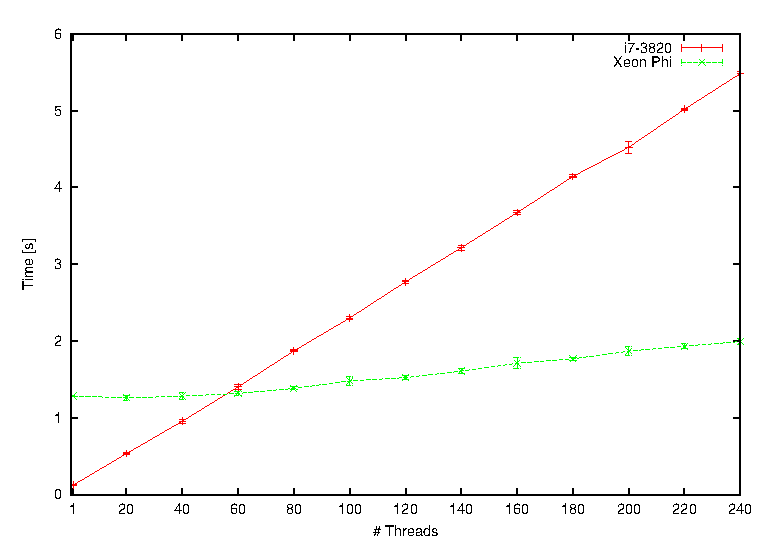
\includegraphics[width=0.9\columnwidth]{../plots/comp_contains/runtime_contains}
	\begin{tikzpicture}
\begin{axis}[
width=3in,
xlabel={\#Threads},
ylabel={Time [s]},
xmin=-10,
xmax=250,
xtick={0,80,...,240},
ytick={0,2000, 4000, 6000, 8000, 10000},
yticklabels={0, 2, 4, 6, 8, 10},
ymin=0,
ymax=10000,
scaled x ticks = false,
scaled y ticks = false,
legend style={at={(0.05,0.95)},anchor=north west, font=\tiny}]

\addplot[mark=*,blue, mark size=1.5]
table[x=Threads,y=lf_xeon,col sep=comma] {../plots/comp_contains/comp_contains.csv}; 
\addlegendentry{Xeon E-1245}

\addplot[color=red,mark=triangle*, mark size=2]
table[x=Threads,y=lf_i7,col sep=comma] {../plots/comp_contains/comp_contains.csv}; 
\addlegendentry{Core i7-3820}

\addplot[color=darkgreen,mark=square*, mark size=1.5]
table[x=Threads,y=lf_xp,col sep=comma] {../plots/comp_contains/comp_contains.csv}; 
\addlegendentry{Xeon Phi}

\end{axis}
\end{tikzpicture}
	\caption{Cache-invalidation assessment}
	\label{fig:comp_contains}
\end{figure}
The previous experiments show that the same workload performs roughly a magnitude better on a Xeon CPU than on Xeon Phi.
Despite the fact that Xeon Phi has many more cores and a higher memory bandwidth.
While there are multiple reasons for this, e.g. different caching architecture, clock frequency, number of write buffers and so on, this experiment should evaluate the impact of cache-invalidation.
% FIXME: multiple reasons before, multiple reasons again... what is going wrong?
There are multiple reasons for these, e.g. cache structure, memory allocation cost, and other problems.
Therefore an experiment was designed to check how Xeon Phi performs, in comparison to other architectures when cache-invalidations are not occurring.
This consists of prepopulating our lock-free concurrent priority queue with 10 million elements, then each thread will do 100'000 lookups in the data structure.
Thereby the structure of the priority queue is unaltered which means no cache-line belonging to the concurrent priority queue should get invalidated.
This experiment was executed with 1 to 240 threads, the run-times, running this experiment on an Intel Core i7-3820, a Xeon CPU and the Xeon Phi, are plotted in Fig.~\ref{fig:comp_contains}.
% FIXME can you improve the second part of the following sentence. It should become 2 sentences, instead of 1.
It can be noted that the runtime on Xeon Phi stays stable up to 60 threads equaling the number of cores, with even more threads it increases only slightly.
Whereas on the other two systems, the execution time increases linearly.
The results show clearly that the invalidation of cache-lines and their consequences have a major impact on the performance on Xeon Phi.
While in the previous experiments it showed a linear increase in execution time when scaling up, in this one the runtime stays almost constant which is close to ideal.

%Also rephrase reson why Xeon Phi is not doing well
This finding is not new, other researchers~\cite{ramos-hoefler-cc-modeling} have shown that a drawback when using a Xeon Phi is that any cache-line invalidation might lead to many cores ending up with dirty cache lines. This is due to fact that it uses a distributed tag directory. Thus, the more hardware cores are used on a concurrent application the probability that at least two threads share a cache line is higher. These dirty cache lines produce expected overhead due to cache invalidations.

Implementing a truly concurrent data structure is a challenging task for many reasons. For instance, even though our implementation is lock-free, it may not be starvation-free. There could be a thread A that when going through the lowest level of the skip list searching for the next un-marked node (i.e. logically undeleted) gets always outrun by some other thread B. This means that thread A can fail repeatedly if the others threads always succeed. Moreover, thread contention may happen if many threads try to logically delete a node (i.e. mark a node). Only one thread will succeed and all the other unsuccessful ones will race to mark
the next available node.\\


\subsection{Operational intensity in different microarchitectures}
% recap of operational intensity
Operational intensity is defined as the ratio of the number of instructions executed to the number of memory accesses~\cite{roger1996science}. If there exist many instructions per memory access, then the program is considered to have a high computational intensity i.e. compute bounded. On the other hand, if there are a small number of instructions are executed per memory access, then the program is considered to have a low computational intensity i.e. memory bounded.

% why we think it matters in our case
Our project goal was to design a simple, yet effective, concurrent priority queue. Thus, we expected to have an operational intensity dominated mainly by the number of memory accesses, and aimed to improve this. Having to move data around, has a different impact on different CPU architectures. We will describe and explain how our data structure behaves on Intel Haswell microarchitecture (Intel Core i7-4558U) and on Sandy BridgeE microarchitecture (Intel Core i7-3820K). 

% Differences between these two microarchitectures
The Intel Haswell microarchiteture is the successor of Ivy Bridge which in turn is the successor of Sandy Bridge. They have several differences but they also share many commonalities. One of the biggest change is the enhancement done on cache level operations. These changes are summarized in \tablename~\ref{tab:haswell_ivy}~\cite{ijcsit2013040321, microarchitecture, haswell_arch}.

%memory hierarchy implemented on the Intel Haswell. The cache bandwidth is doubled and its memory system can now perform two loads and one store per cycle. The Haswell's L1 load bandwidth is of 64 bytes/cycle, its L1 store bandwidth is of 32 bytes/cycle and also L2 bandwidth to L1 has doubled (from 32 bytes/cycle to 64 bytes/cycle). Other relevant improvements are the ones related to the Translation Look-aside Buffer (TLB) which in Haswell has access to 2M shared pages. The page entry also doubled in Haswell as well as the associativity; It went from a 4-way associative TLB in Ivy Bridge to a 8-way associative TLB in Haswell. 

\begin{table}[ht]
\footnotesize
\begin{tabular}{|l|l|l|ll}
\cline{1-3}
\multicolumn{1}{|c|}{\textbf{Metric}} & \multicolumn{1}{c|}{\textbf{Sandy BridgeE}} & \multicolumn{1}{c|}{\textbf{Haswell}} &  &  \\ \cline{1-3}
L1 Load Bandwidth                     & 32 Bytes/cycle                           & 64 Bytes/cycle                        &  &  \\ \cline{1-3}
L1 Store bandwidth                    & 16 Bytes/cycle                           & 32 Bytes/cycle                        &  &  \\ \cline{1-3}
L2 Bandwidth to L1                    & 32 Bytes/cycle                           & 64 Bytes/cycle                        &  &  \\ \cline{1-3}
L2 Unified TLB                        & 4K:512, 4-way                            & 4k+2M shared: 1024, 8-way             &  &  \\ \cline{1-3}
\end{tabular}
\caption{Cache operation differences between Intel Haswell and Intel SandyBridgeE}
\label{tab:haswell_ivy}
\end{table}

% describe cache structure
In addition to core cache size, latency, and bandwidth improvements, the Intel Haswell microarchitecture has also improved its ICache prefetch algorithms, and the way it handles conflicts. It uses hardware transactions i.e. it uses hardware to keep track of which cache lines have been read from and which have been written to. L1 cache tracks addresses read/written from/to respectively in the transactional region and it may evict address but without loss of tracking. Data conflicts occur if at least one request is doing a write, but it is detected at cache line granularity using existing cache coherence protocol~\cite{rajwar_qconsf2012,dk_haswell}.

While running our priority queue benchmark on these two different architectures, we observed different behaviors. The running times when using an Intel IvyBridge processor dramatically increase due to a higher number of instructions and cache misses. Everytime we need to perform an insertion, we first have to search for the adequate place within the skip list. The average of the skip list nodes fit in a 64-byte cache line but the ones containing pointers in upper levels do not. On the other hand, when we used an Intel Haswell processor, running times were much less than in the Sandy BridgeE processor. This is mainly due to the improvements done on cache operations. In this case, our data structure can take advantage of such improvements by loading more skip list nodes into the caches that can also be used by other threads.

% explain data + graph + core architecture
\begin{figure}[t]
	\centering
  	%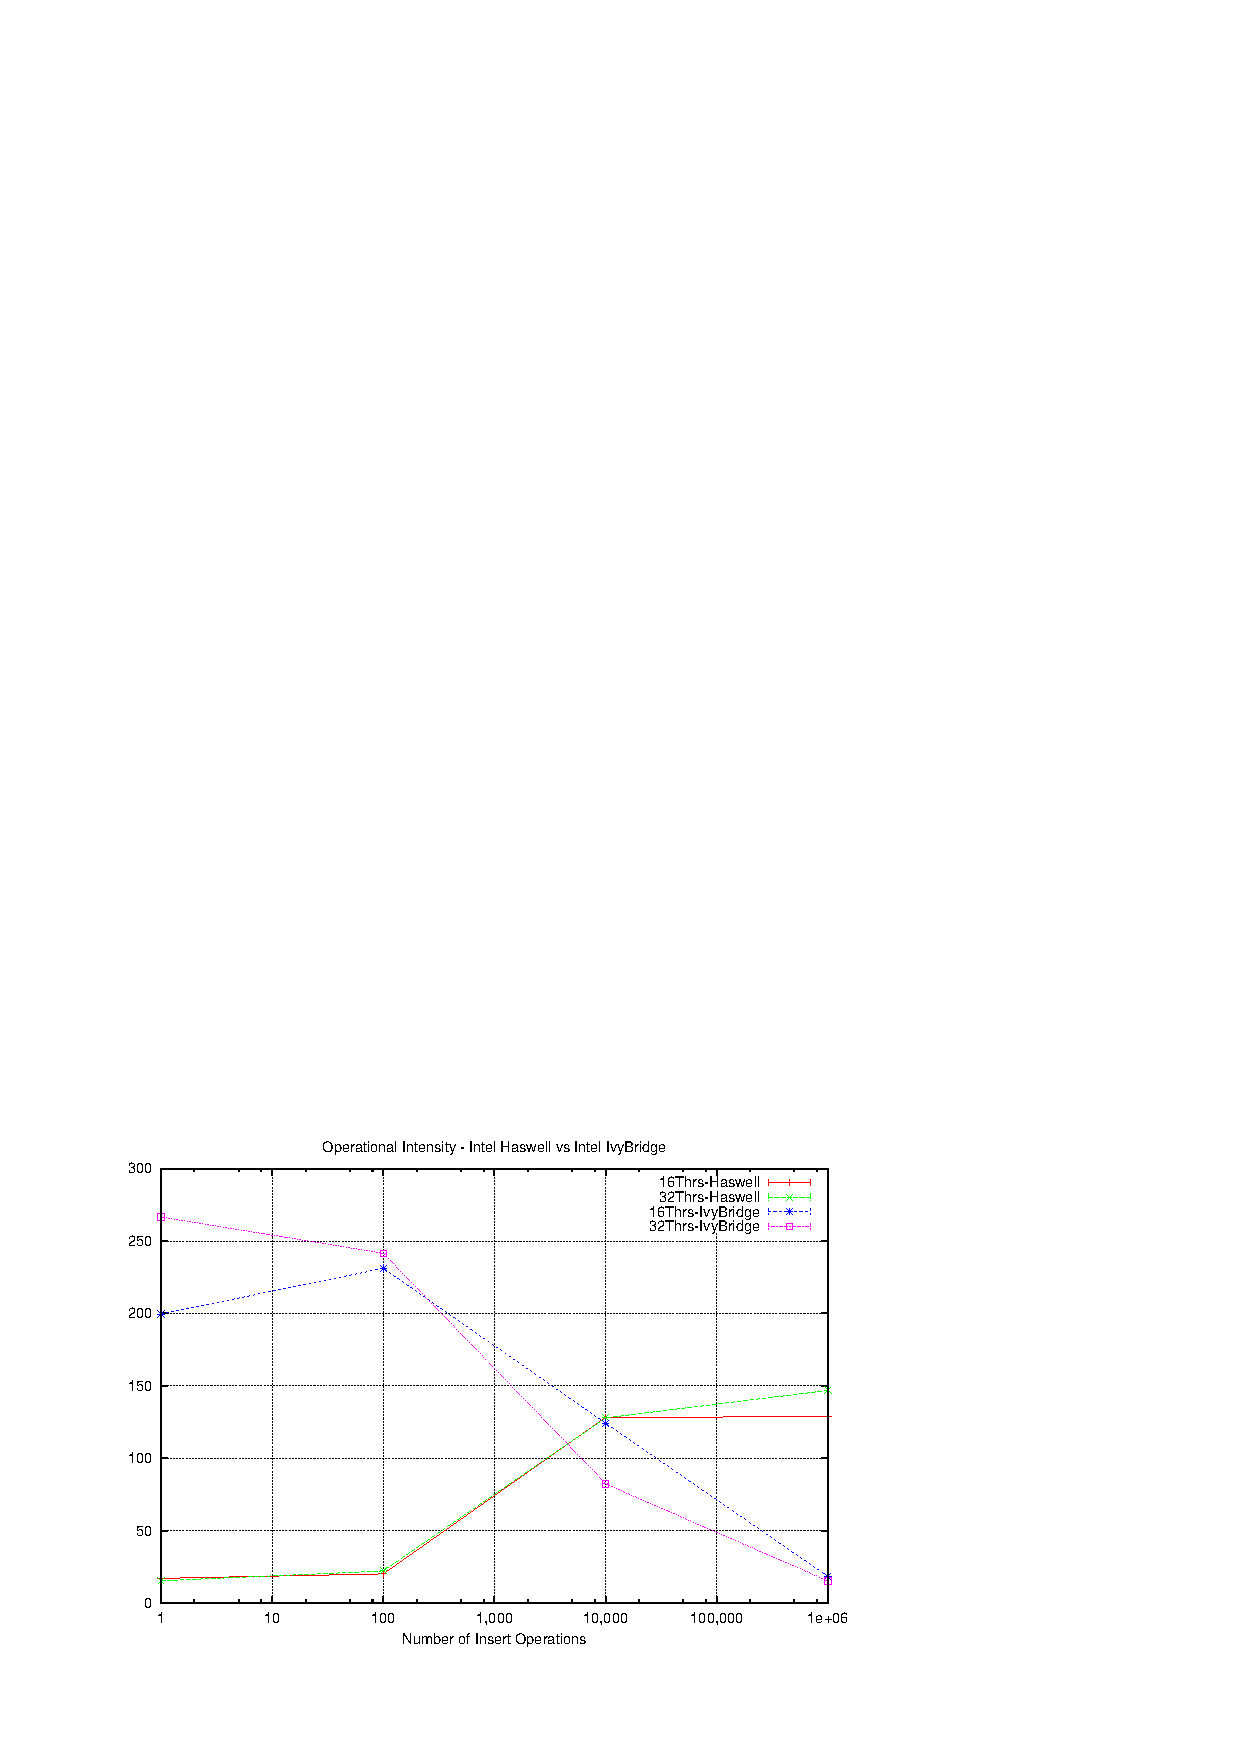
\includegraphics[scale=0.3]{../plots/haswell-ivybridge/haswell_ivybridge.pdf}
	\begin{tikzpicture}
\begin{axis}[
width=3in,
xlabel={Number of operations},
ylabel={Operations Intensity},
%xmin=-10,
%xmax=250,
xmode=log,
xtick={1, 100, 10000, 1000000},
ytick={0, 5, 10, 15, 20},
ymin=0,
ymax=20,
scaled x ticks = false,
scaled y ticks = false,
legend style={at={(0.95,0.95)},anchor=north east, font=\tiny}]

\addplot[mark=*,blue, mark size=1.5, smooth]
table[x=Ops,y=16t_has,col sep=comma] {../plots/haswell-ivybridge/haswell_ivybridge.csv}; 
\addlegendentry{16\,Thrs Haswell}

\addplot[color=red,mark=triangle*, mark size=2, smooth]
table[x=Ops,y=32t_has,col sep=comma] {../plots/haswell-ivybridge/haswell_ivybridge.csv}; 
\addlegendentry{32\,Thrs Haswell}

\addplot[color=orange,mark=square*, mark size=1.5, smooth]
table[x=Ops,y=16t_ivy,col sep=comma] {../plots/haswell-ivybridge/haswell_ivybridge.csv}; 
\addlegendentry{16\,Thrs Ivy}

\addplot[color=darkgreen,mark=diamond*, mark size=1.5, smooth]
table[x=Ops,y=32t_ivy,col sep=comma] {../plots/haswell-ivybridge/haswell_ivybridge.csv}; 
\addlegendentry{32\,Thrs Ivy}

\end{axis}
\end{tikzpicture}
	\caption{Op. Intensity in Intel Haswell and Intel Sandy BridgeE microarchitectures}
	\label{fig:haswell_ivybridge}
\end{figure}

Fig.~\ref{fig:haswell_ivybridge} shows how operational intensity behaves when running different amounts of insert operations over such micro-architectures. It can be noted that when performing a small number of operations, our data structure is CPU bounded on an Sandy BridgeE processor, but memory bounded on a Haswell processor. This is because in the former we have a small number of cache-misses against a really high number of instructions whether in the latter we observed a low operational intensity because we need less number of instructions for performing such tasks. When we increase the number of operations, the Sandy BridgeE processor gets many more cache-misses compared to the Haswell one. Thus, in the former one our data structure becomes memory bounded and in the latter one CPU bounded.

%Another problem could arise when some node physically deletes a node that other threads are still using. This will lead into repeated \textit{compareAndSet} failures.
%Doing experiments with different microarchitectures has lead us to deeper understanding of the tradeoffs in each of them. For instance, utilizing Xeon Phi for our data structure means that every time a thread updates a node, the operation will also be copied into the remote caches due to the tag-directory cache with explicit updates present on Xeon Phi. Being able to update all CPUs at once does not show any performance gain because multiple writes cause more traffic and more invalidations which is a more expensive operation on Xeon Phi. On the other hand, our implementation gains performance in a microarchitecture with bigger caches size (e.g. Intel Haswell). This hardware enhancement helps us change the operational intensity of our data structure, making it compute bound and not memory bound any more. Thus, we can load more elements each time improving its spatial locality.


\section{Conclusions}
\label{sec:con}
We presented lock-free concurrent priority queue based on a skip list. The implementation was evaluated on a common x86 CPU and more importantly on a Xeon Phi MIC. The results show that our implementation is competitive in comparison to asses baseline implementations. On the MIC architecture all tested implementations are below our expectations and are unable to take advantage of the hardware. Our lock-free implementation suffers mostly from the overhead due to the cache-consistency protocol.

%\section{Further comments}

%Here we provide some further tips.

%\mypar{Further general guidelines}

%\begin{itemize}
%\item For short papers, to save space, I use paragraph titles instead of
%subsections, as shown in the introduction.
%
%\item It is generally a good idea to break sections into such smaller
%units for readability and since it helps you to (visually) structure the story.
%
%\item The above section titles should be adapted to more precisely
%reflect what you do.
%
%\item Each section should be started with a very
%short summary of what the reader can expect in this section. Nothing
%more awkward as when the story starts and one does not know what the
%direction is or the goal.
%
%\item Make sure you define every acronym you use, no matter how
%convinced you are the reader knows it.
%
%\item Always spell-check before you submit (to me in this case).
%
%\item Be picky. When writing a paper you should always strive for very
%high quality. Many people may read it and the quality makes a big difference.
%In this class, the quality is part of the grade.
%
%\item Books helping you to write better: \cite{Higham:98} and \cite{Strunk:00}.
%
%\item Conversion to pdf (latex users only): 
%
%dvips -o conference.ps -t letter -Ppdf -G0 conference.dvi
%
%and then
%
%ps2pdf conference.ps
%\end{itemize}
%
%\mypar{Graphics} For plots that are not images {\em never} generate
%jpeg, gif, bmp, tif. Use eps, which means encapsulate postscript. It
%scalable since it is a vector graphic description of your graph. E.g.,
%from Matlab, you can export to eps.
%
%Here is an example of how to get a plot into latex
%(Fig.~\ref{fftperf}). Note that in this plot the text should be
%a little bit larger. In particular, the labels are too small!
%
%\begin{figure}\centering
%  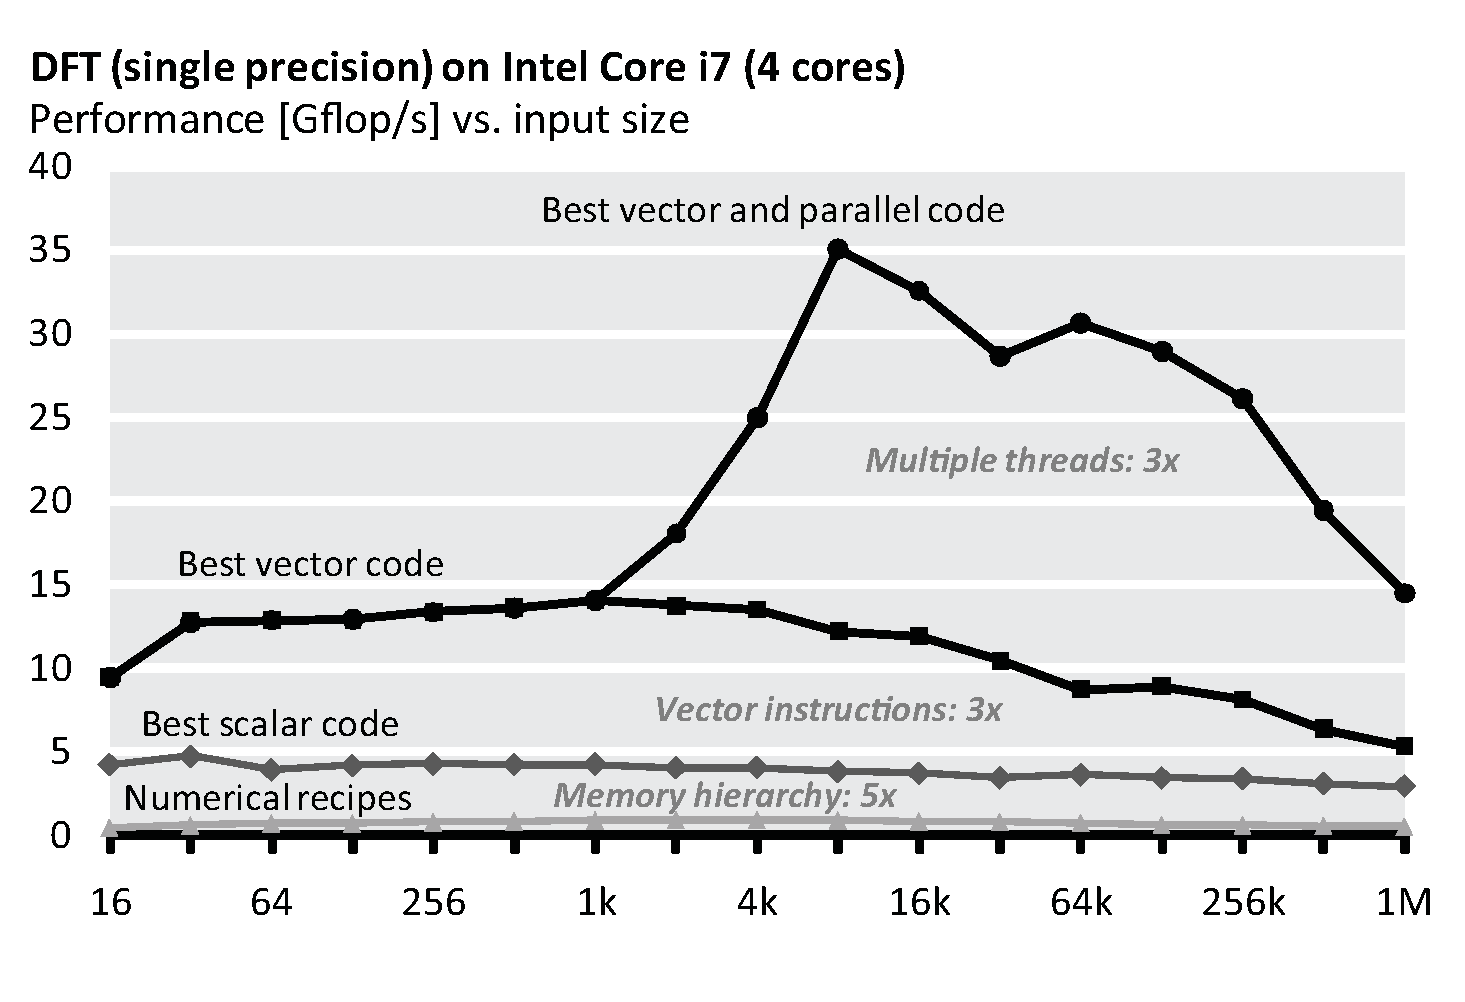
\includegraphics[scale=0.33]{dft-performance.eps}
%  \caption{Performance of four single precision implementations of the
%  discrete Fourier transform. The operations count is roughly the
%  same. {\em The labels in this plot are too small.}\label{fftperf}}
%\end{figure}



% References should be produced using the bibtex program from suitable
% BiBTeX files (here: bibl_conf). The IEEEbib.bst bibliography
% style file from IEEE produces unsorted bibliography list.
% -------------------------------------------------------------------------
\bibliographystyle{IEEEbib}
\bibliography{bibl_conf}

\end{document}

